\documentclass[11pt]{report}

% For including image file
\usepackage{graphicx, color}

% For including collection of image
%\usepackage{subcaption}

% For generating hyper links

% For coloring text
\usepackage{xcolor}

%\usepackage{hyperref}
\usepackage[linkbordercolor=white, colorlinks=true, urlcolor=black, linkcolor=black]{hyperref}

% Margin of the page
\usepackage[top=0.5in, bottom=1in, left=1in, right=1in]{geometry}

%For adding nomenclature
%\usepackage{nomencl}
%\makenomenclature
%\renewcommand{\nomname}{Annotation}

% For cover page tikz image 
%\usepackage{tikz}
%\usetikzlibrary{calc}

% For including a piece of code
%\usepackage{listings}

% Images folder
%\graphicspath{{Images/}}

\usepackage{titlesec}

\titleformat{\chapter}[display]
{\normalfont\Large\filcenter\sffamily}
{\vspace*{\fill}
 \titlerule[1pt]%
 \vspace{1pt}%
 \titlerule
 \vspace{1pc}%
 \LARGE\MakeUppercase{\chaptertitlename}~\thechapter}
{1pc}
{\titlerule\Huge}
[\vspace*{\fill}\newpage]

\titlespacing*{\chapter}{0pt}{0pt}{0pt}

\titleformat{name=\chapter,numberless}[display]
{\normalfont\Large\filcenter\sffamily}
{}
{0pt}
{\titlerule[1pt]\Huge}
[\titlerule]

\usepackage{pdfpages}

\begin{document}

\tableofcontents

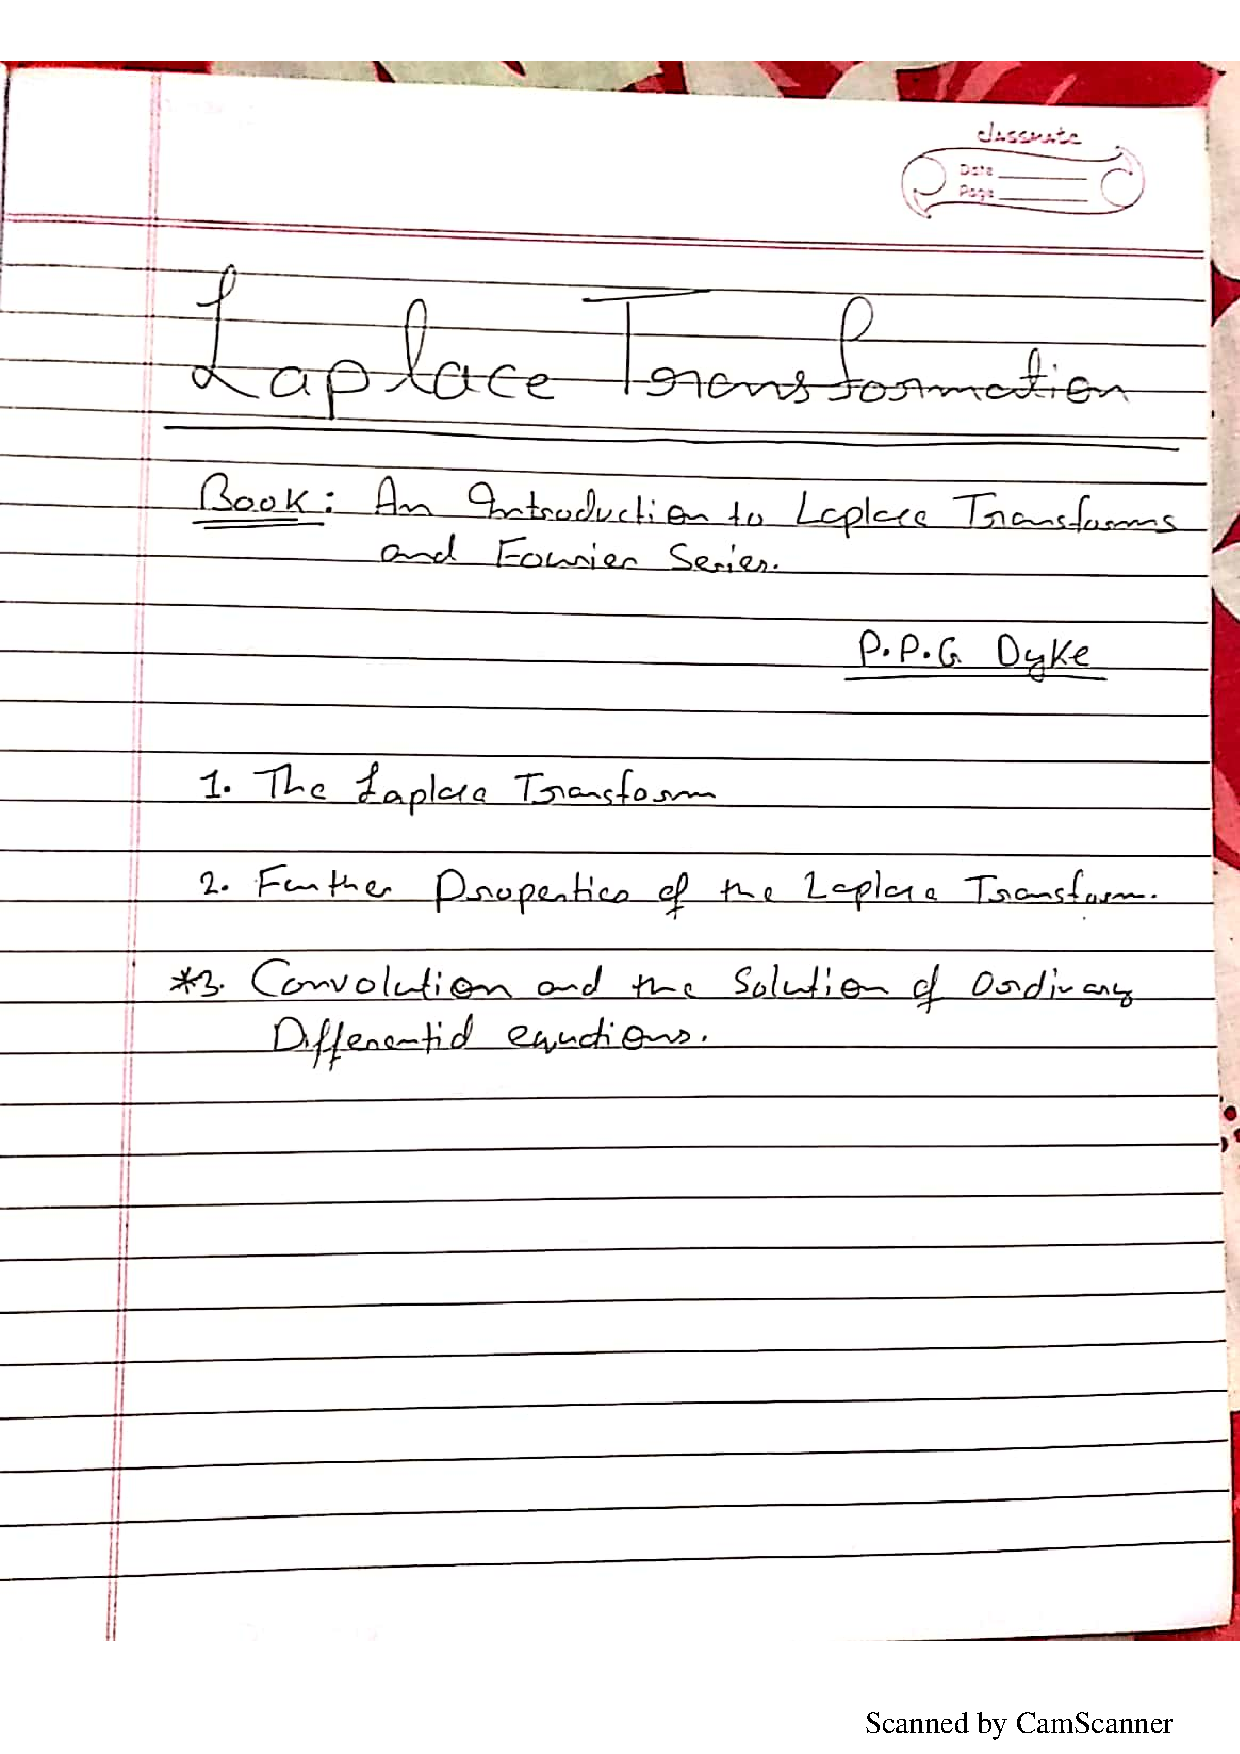
\includepdf[page=-]{./raw_files/cover.pdf}

\chapter{The Laplace Transform}
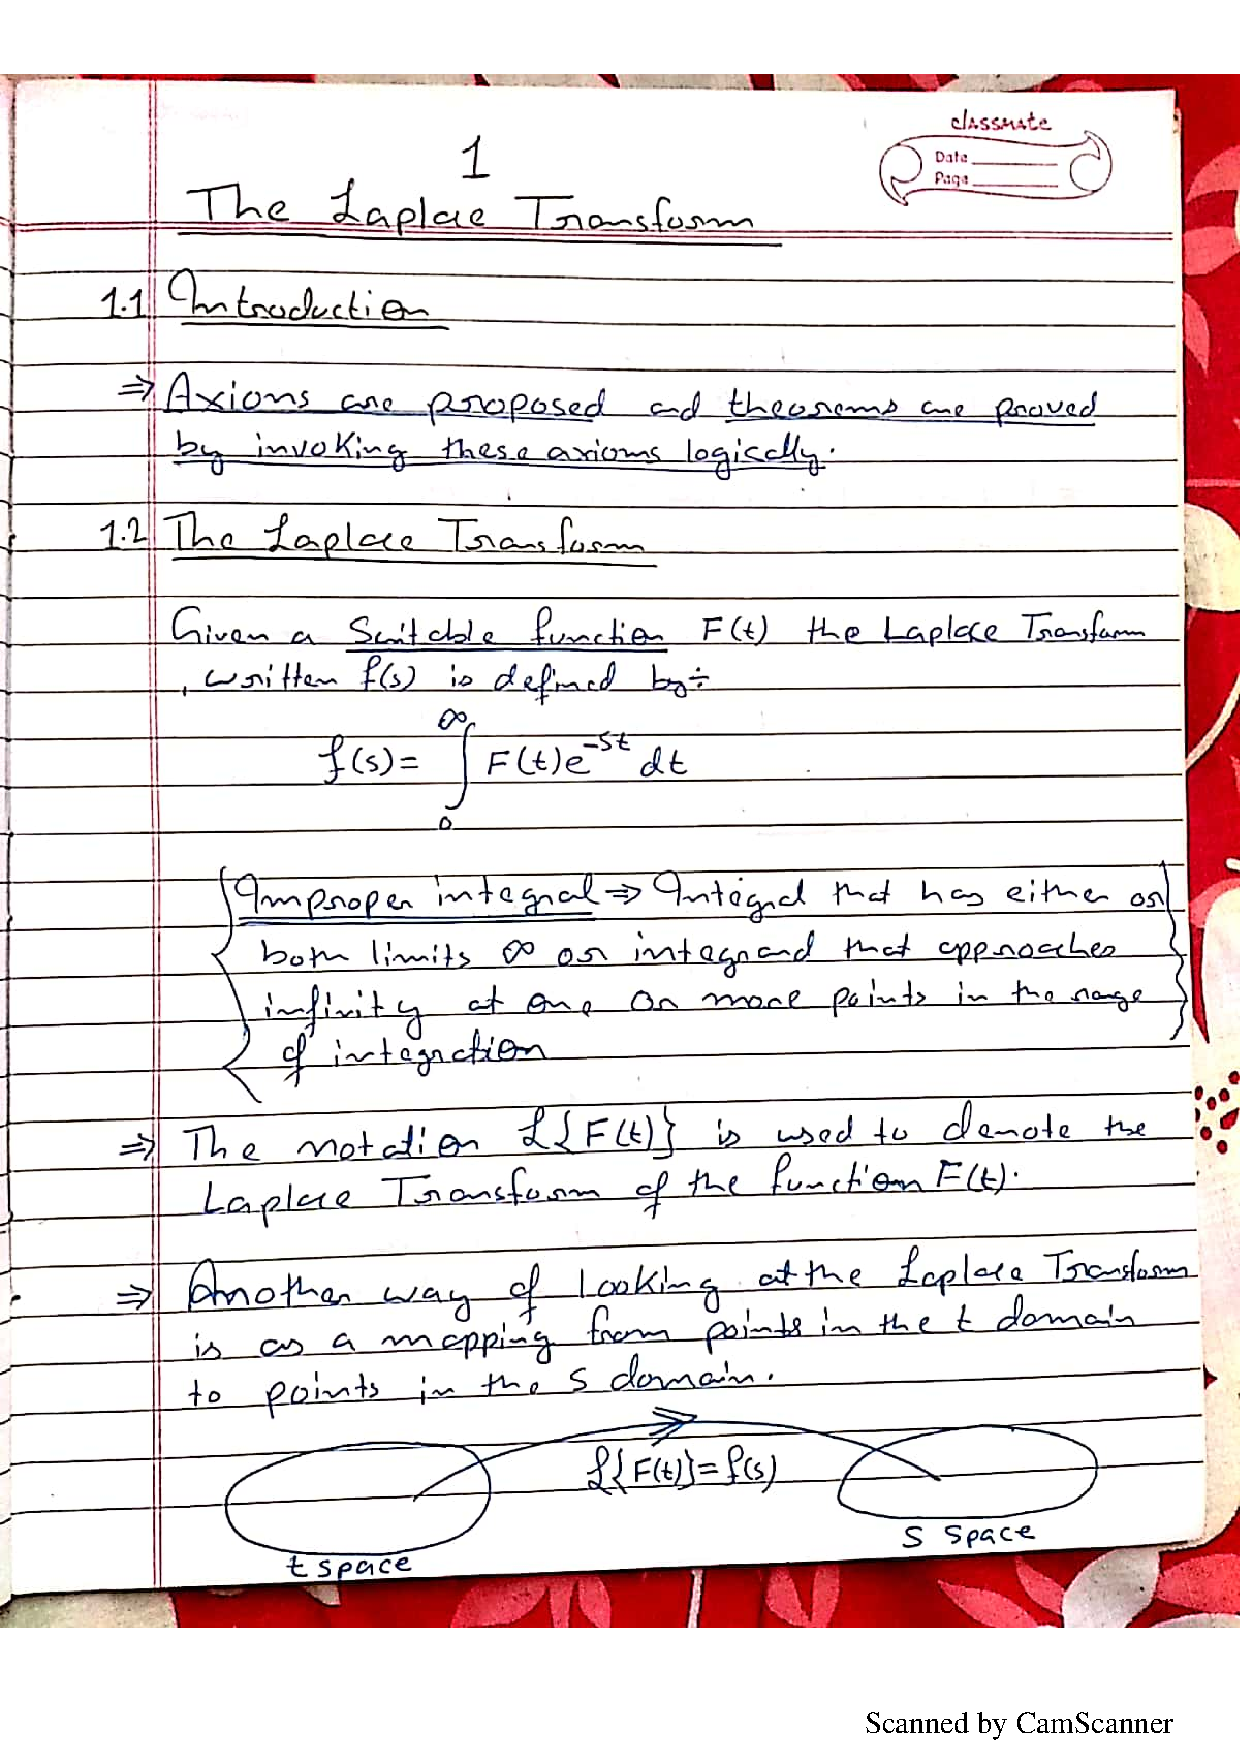
\includepdf[page=-]{./raw_files/1.pdf}

\chapter{Furture Properties of the Laplace Transforms}
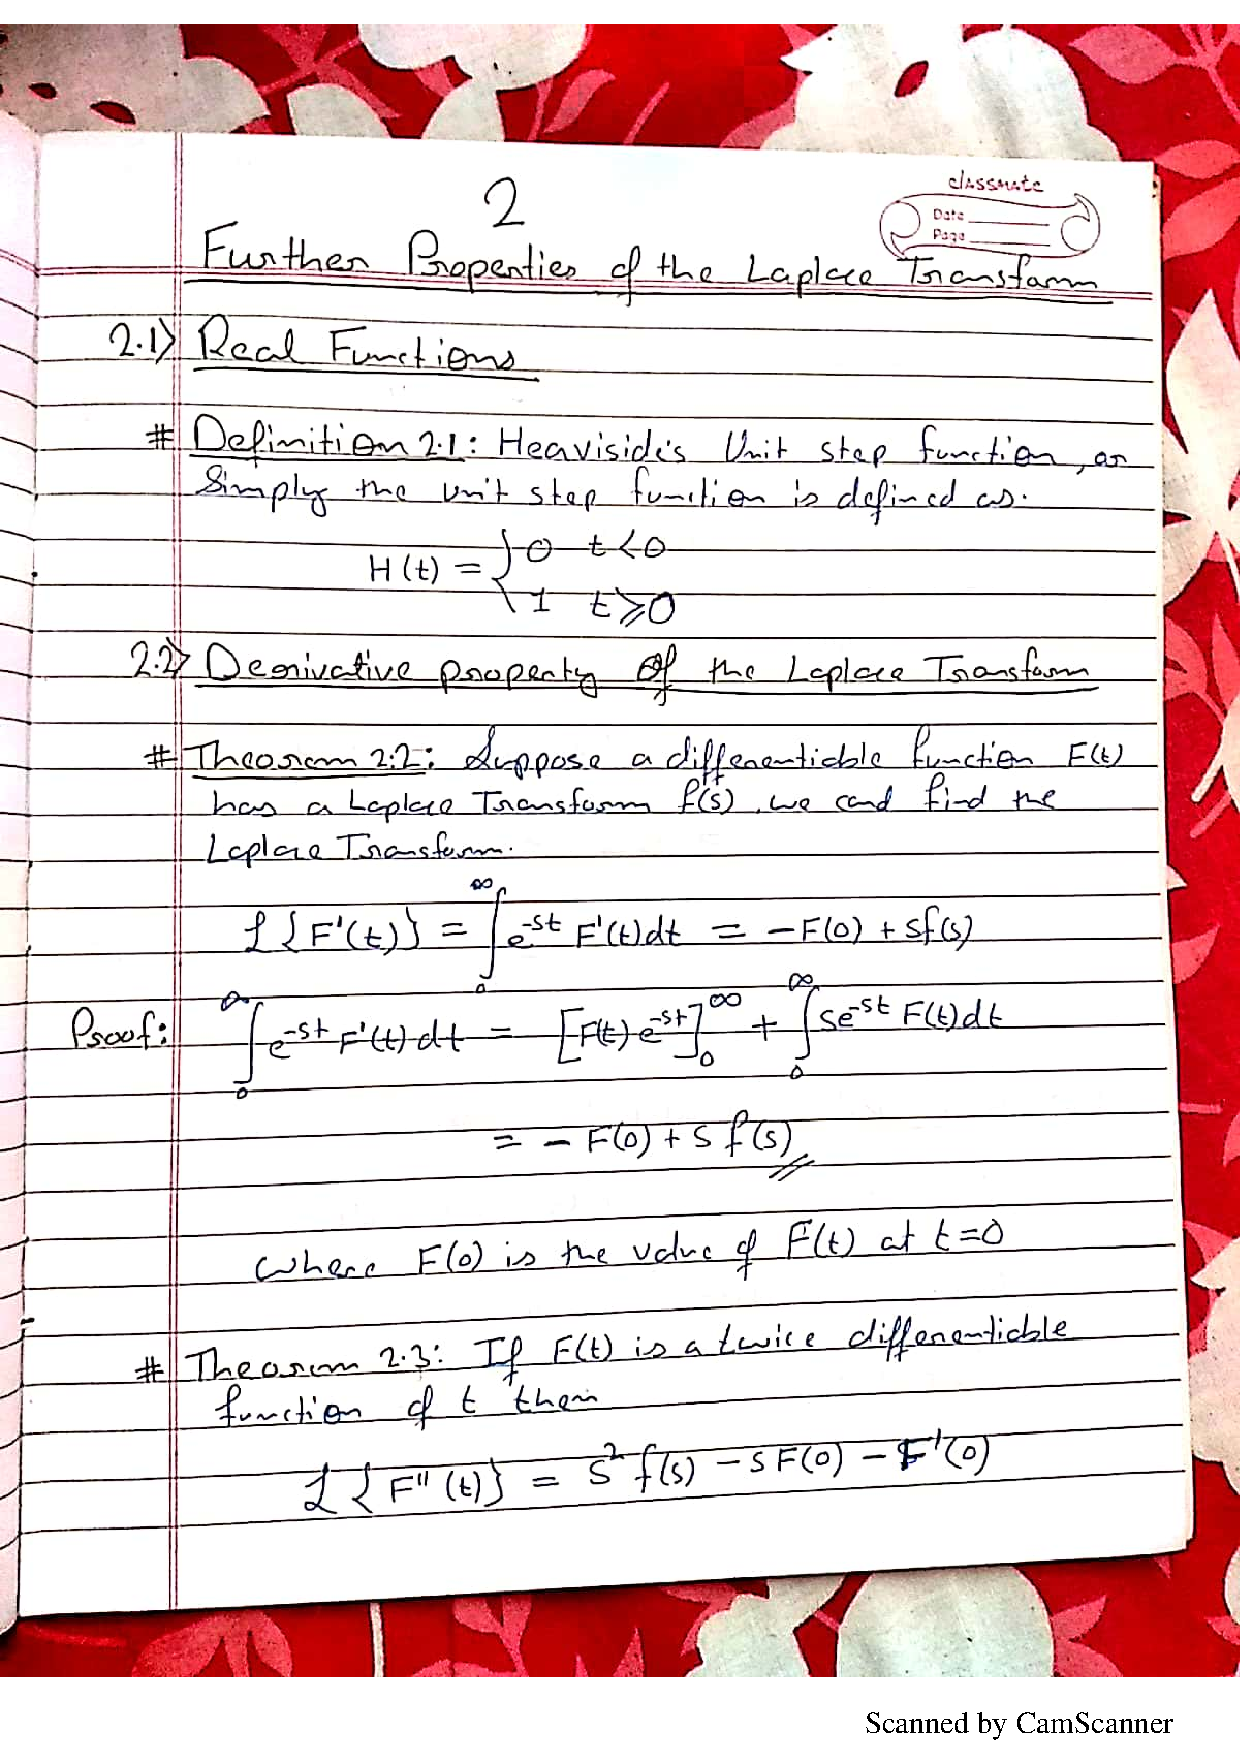
\includepdf[page=-]{./raw_files/2.pdf}

\chapter{Convolution and the Solution of Ordinary Differential Equation}
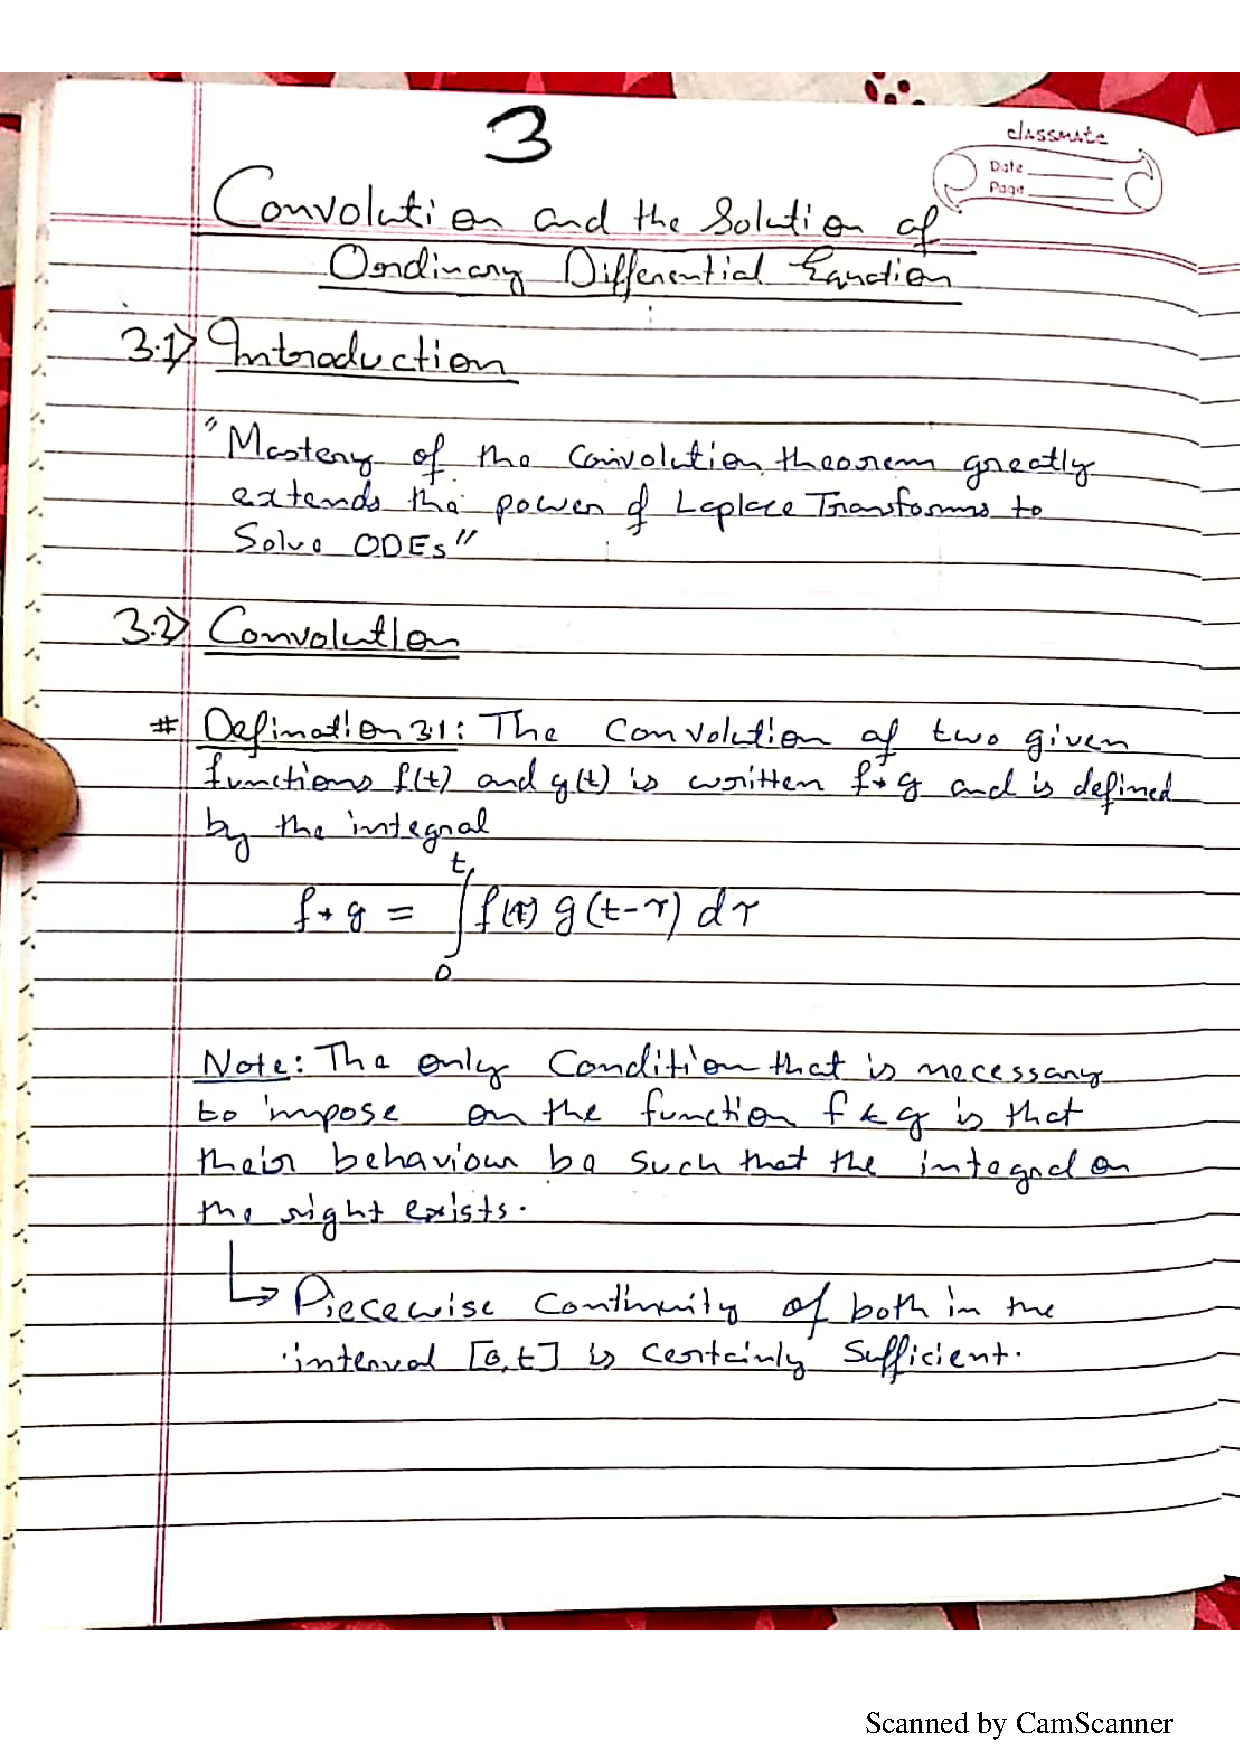
\includepdf[page=-]{./raw_files/3.pdf}

\end{document}